\documentclass[11pt,a4paper]{article}
\usepackage[margin=19mm,headheight=14pt,headsep=7mm,footskip=10mm]{geometry}
\usepackage{amsmath,amssymb}
\usepackage{newtxtext,newtxmath}
\usepackage{xcolor,booktabs,tabularx,array,graphicx,enumitem,fancyhdr}
\usepackage[colorlinks=true,linkcolor=blue!45!black,urlcolor=blue!45!black]{hyperref}
\definecolor{navy}{HTML}{17354D}
\definecolor{teal}{HTML}{087E83}
\definecolor{pale}{HTML}{EFF5F7}
\setlength{\parindent}{0pt}
\setlength{\parskip}{5pt}
\setlength{\abovedisplayskip}{6pt}
\setlength{\belowdisplayskip}{6pt}
\setlength{\abovedisplayshortskip}{3pt}
\setlength{\belowdisplayshortskip}{3pt}
\renewcommand{\baselinestretch}{1.06}
\setlist[itemize]{leftmargin=16pt,itemsep=3pt,topsep=3pt}
\setlist[enumerate]{leftmargin=18pt,itemsep=3pt,topsep=3pt}
\pagestyle{fancy}\fancyhf{}
\fancyhead[L]{\small\textcolor{navy}{WELCH MI \enspace / \enspace PERSONAL STUDY GUIDE}}
\fancyhead[R]{\small Daniel Zhao}
\fancyfoot[L]{\small\textcolor{navy}{Derivations, evidence and interpretation}}
\fancyfoot[R]{\small\thepage\ / 12}
\renewcommand{\headrulewidth}{0.3pt}
\newcommand{\E}{\operatorname{E}}
\newcommand{\Var}{\operatorname{Var}}
\newcommand{\Cov}{\operatorname{Cov}}
\newcommand{\Ih}{\widehat I}
\newcommand{\Vh}{\widehat V}
\newcommand{\Dh}{\widehat\Delta}
\newcommand{\SEh}{\widehat{\mathrm{SE}}}
\newcommand{\ind}{\mathbf 1}
\newcommand{\subhead}[1]{\par\medskip\textbf{\textcolor{navy}{#1}}\par\smallskip}
\newcommand{\takeaway}[1]{\par\medskip\noindent\colorbox{pale}{\parbox{\dimexpr\linewidth-2\fboxsep\relax}{\textbf{Remember:} #1}}\par}
\newcommand{\source}[1]{\par\smallskip{\footnotesize\textcolor{navy}{Thesis reference: #1.}}}
\newcommand{\topic}[2]{\clearpage\pdfbookmark[0]{#1}{topic\thepage}{\Large\bfseries\color{navy}#1}\par\smallskip{\itshape #2}\par\medskip}
\hypersetup{pdftitle={Welch MI: Main Derivations and Experimental Results},pdfauthor={Daniel Zhao},pdfsubject={Personal study guide to the current Welch MI thesis}}
\begin{document}
\pdfbookmark[0]{1. Question, notation and method}{topic1}

{\LARGE\bfseries\color{navy}Welch MI: derivations and results}\par
{\large A 12-page guide for understanding your thesis}\par
{\small Based on the thesis version of 6 November 2026. All MI values use natural logarithms and are measured in nats.}
\par{\small\textcolor{navy}{Derivations: pp. 2--7 \quad Design: p. 8 \quad Results: pp. 9--11 \quad Application: p. 12}}

\subhead{1. What question are we answering?}
Within each population, two categorical variables \(X\) and \(Y\) have a joint probability table. We want to know whether their association, measured by mutual information (MI), differs between populations \(P\) and \(Q\):
\[
 \Delta=I(P)-I(Q),\qquad H_0:\Delta=0,\qquad H_1:\Delta\ne0.
\]
The samples from \(P\) and \(Q\) are independent. This does \emph{not} require \(X\) and \(Y\) to be independent within either population. Equal MI also does not require equal probability tables: different category frequencies or association patterns can give the same MI.

\subhead{The whole method in one chain}
For cell probabilities \(p_{ij}\), row margins \(p_{i+}\) and column margins \(p_{+j}\), define
\[
 s_P(i,j)=\log\frac{p_{ij}}{p_{i+}p_{+j}},\qquad
 I(P)=\sum_{i,j}p_{ij}s_P(i,j).
\]
Here \(s_P\) denotes pointwise MI throughout this guide. It can be negative in an individual cell, while its population average \(I(P)\) is nonnegative. A sample gives empirical probabilities \(\widehat p_{ij}=N_{ij}/n_P\) and a plug-in estimate \(\Ih(P)\). With \(d=(r-1)(c-1)\), the tests share
\[
 \Dh=\left\{\Ih(P)-\frac{d}{2n_P}\right\}
       -\left\{\Ih(Q)-\frac{d}{2n_Q}\right\},\quad
 \SEh^2=\frac{\Vh(P)}{n_P}+\frac{\Vh(Q)}{n_Q},\quad
 T=\frac{\Dh}{\SEh}.
\]
Wald compares \(T\) with the standard normal distribution. Expanded Welch compares the same \(T\) with a Student \(t\) distribution whose degrees of freedom are estimated from the tables. Its larger cutoff reduces rejection. The thesis asks when this reduction improves false-positive rates and how much power it costs.

\subhead{The variance quantities you need to keep separate}
\begin{tabularx}{\linewidth}{@{}lX@{}}\toprule
Quantity & Meaning\\\midrule
\(V(P)=\Var_P\{s_P(X,Y)\}\) & Variation in pointwise MI across outcomes in a population.\\
\(\Vh(P)\) & An estimate of \(V(P)\) from one whole sampled table.\\
\(V(P)/n_P\) & First-order approximation to \(\Var\{\Ih(P)\}\).\\
\(\Var\{\Vh(P)\}\) & Variation of the variance estimate across repeated whole tables.\\
\(\tau^2(P)\) & Variance of the sensitivity \(g_P\), giving \(\Var(\Vh)\approx\tau^2/n_P\).\\\bottomrule
\end{tabularx}

\takeaway{The new contribution concerns how the estimated variance changes between samples. The MI difference and standard error are shared with Wald.}
\source{Chapters 1, 3 and 4. Pages 2--7 below derive the method; pages 8--12 explain the experiments and findings}

\topic{2. Why MI has variance \texorpdfstring{\(V/n\)}{V/n}, and why we correct bias}{The first Taylor expansion explains the shared standard error.}

\subhead{Expand MI around the population table}
Write \(\delta_{ij}=\widehat p_{ij}-p_{ij}\), so \(\sum_{i,j}\delta_{ij}=0\). The general first-order Taylor formula is \(f(x+h)\approx f(x)+\nabla f(x)^\mathsf{T}h\). Here \(f\) is MI, the expansion point is \(P\), the new value is \(\widehat P\), and the change is \(\delta\).

Expressing MI as joint and marginal probability sums gives
\[
 I(P)=\sum_{i,j}p_{ij}\log p_{ij}
       -\sum_i p_{i+}\log p_{i+}-\sum_j p_{+j}\log p_{+j}.
\]
Since the derivative of \(u\log u\) is \(1+\log u\), the coefficient of a change in cell \((i,j)\) is
\[
 (1+\log p_{ij})-(1+\log p_{i+})-(1+\log p_{+j})=s_P(i,j)-1.
\]
The constant disappears when multiplied by the cell errors and summed:
\[
 \Ih(P)-I(P)\approx\sum_{i,j}\{s_P(i,j)-1\}\delta_{ij}
 =\sum_{i,j}s_P(i,j)\delta_{ij}.
\]
For independent observations \(Z_a=(X_a,Y_a)\), substituting the empirical proportions turns this into an average:
\[
 \Ih(P)-I(P)\approx\frac1n\sum_{a=1}^n\{s_P(Z_a)-I(P)\}.
\]
Each summand has mean zero and variance \(V(P)\). Independence removes cross-observation covariances, so
\[
 \Var\{\Ih(P)\}\approx\frac{1}{n^2}\sum_{a=1}^n V(P)=\boxed{\frac{V(P)}n}.
\]
This uses fixed categories, positive population probabilities and a nonzero first-order variance. The empirical estimate is
\[
 \Vh(P)=\sum_{i,j:\widehat p_{ij}>0}\widehat p_{ij}
                  \{\widehat s_P(i,j)-\Ih(P)\}^2.
\]

\subhead{The leading bias is a second-order effect}
The linear error above has mean zero, so it does not explain finite-sample bias. For entropy with \(m\) positive-probability categories, the second derivative of \(-u\log u\) is \(-1/u\). Using \(\Var(\widehat p_i)=p_i(1-p_i)/n\), the quadratic term gives
\[
 \E\{\widehat H-H\}\approx-\frac12\sum_i\frac{p_i(1-p_i)}{np_i}
 =-\frac{m-1}{2n}.
\]
Because \(I=H(X)+H(Y)-H(X,Y)\), the leading MI bias is
\[
 \frac{-(r-1)-(c-1)+(rc-1)}{2n}=\boxed{\frac{(r-1)(c-1)}{2n}}.
\]
Subtracting this fixed correction changes the estimated MI but not its sampling variance. If \(n_P=n_Q\), the corrections cancel exactly from \(\Dh\). Unequal remaining biases can still shift the difference.

\takeaway{\(V/n\) comes from linear sampling error; the bias correction comes from quadratic error. Neither calculation guarantees accuracy in sparse samples.}
\source{Sections 2.2--2.3 and Chapter 3}

\topic{3. Deriving the variance sensitivity \texorpdfstring{\(g_P(x,y)\)}{gP(x,y)}}{The central calculation tracks changes in both probability weights and pointwise-MI values.}

\subhead{Move a little probability towards one outcome}
Use the path \(P_\varepsilon=(1-\varepsilon)P+\varepsilon\delta_{(x,y)}\), where \(\delta_{(x,y)}\) puts all mass in the selected cell. Define the sensitivity
\[
 g_P(x,y)=\left.\frac{\mathrm d}{\mathrm d\varepsilon}V(P_\varepsilon)\right|_0.
\]
Along this path, \(p'_{ij}=\ind\{i=x,j=y\}-p_{ij}\), with analogous row and column derivatives. Differentiating the three logarithms in pointwise MI gives
\[
 s'_P(i,j)=\frac{\ind\{i=x,j=y\}}{p_{ij}}
          -\frac{\ind\{i=x\}}{p_{i+}}
          -\frac{\ind\{j=y\}}{p_{+j}}+1.
\]
The constant is \(-1+1+1\). For MI, the product rule gives
\[
 I'=\sum_{i,j}p'_{ij}s_P(i,j)+\sum_{i,j}p_{ij}s'_P(i,j)
    =s_P(x,y)-I(P),
\]
because the second sum is \(1-1-1+1=0\).

\subhead{Differentiate the second moment and subtract \(I^2\)}
Define row and column conditional means, which collect the margin effects:
\[
 R_x=\frac{\sum_jp_{xj}s_P(x,j)}{p_{x+}},\qquad
 C_y=\frac{\sum_ip_{iy}s_P(i,y)}{p_{+y}}.
\]
For \(V(P)=\E_P(s_P^2)-I(P)^2\), the two product-rule terms are
\begin{align*}
 \left.\frac{\mathrm d}{\mathrm d\varepsilon}\E_{P_\varepsilon}(s_{P_\varepsilon}^2)\right|_0
 &=s_P(x,y)^2-\E_P(s_P^2)
   +2\{s_P(x,y)-R_x-C_y+I(P)\}.
\end{align*}
The first pair comes from changing the cell weights. The bracket comes from changing the scores themselves: the indicators select the cell, its row and its column. Subtract \(2I(P)I'\) and use \(\E_P(s_P^2)=V(P)+I(P)^2\). Completing the square yields
\[
 \boxed{\begin{aligned}
 g_P(x,y)={}&\{s_P(x,y)-I(P)\}^2-V(P)\\
            &+2\{s_P(x,y)-R_x-C_y+I(P)\}.
 \end{aligned}}
\]
The first line is the sensitivity of a variance if the scores were fixed. The second line is essential because estimating a new table changes the log ratios and their margins.

\subhead{Why its mean is zero}
The first line averages to \(V(P)-V(P)=0\). Averaging either conditional mean gives MI: \(\E(R_X)=\E(C_Y)=I(P)\). Thus
\[
 \E_P(g_P)=0+2\{I(P)-I(P)-I(P)+I(P)\}=0.
\]
Consequently \(\tau^2(P)=\Var_P(g_P)=\sum_{x,y}p_{xy}g_P(x,y)^2\).

\takeaway{Treating the observed pointwise-MI scores as fixed would omit the margin and score changes. Those changes distinguish the expanded calculation.}
\source{Section 4.2. The notation \(R_x,C_y\) here abbreviates its explicit conditional means}

\topic{4. From \texorpdfstring{\(g_P\)}{gP} to component degrees of freedom}{Linearise the variance estimator, then match two sampling moments.}

\subhead{Turn observation-level sensitivities into sampling variation}
The empirical table is an average of one-observation tables:
\[
 \widehat P-P=\frac1n\sum_{a=1}^n(\delta_{Z_a}-P).
\]
For the first-order Taylor expansion of \(V\), the expansion point is \(P\), the new table is \(\widehat P\), and the change is the average above. The derivative is linear in this change, so
\[
 \Vh(P)-V(P)\approx\frac1n\sum_{a=1}^ng_P(Z_a).
\]
Since \(\E(g_P)=0\) and the observations are independent,
\[
 \boxed{\E\{\Vh(P)\}\approx V(P),\qquad
        \Var\{\Vh(P)\}\approx\frac{\tau^2(P)}n.}
\]
These are approximations to two different moments. Predicting the variance accurately does not imply that the sampling mean is close to \(V(P)\).

\subhead{Why the moment-matching formula is \(2\mu^2/\sigma^2\)}
Let \(\mu=\E(\Vh)\), \(\sigma^2=\Var(\Vh)\), and approximate \(\Vh\) by \(\mu U/\nu\), with \(U\) following a chi-squared distribution with \(\nu\) degrees of freedom. Since \(\E(U)=\nu\) and \(\Var(U)=2\nu\),
\[
 \E(\mu U/\nu)=\mu,\qquad
 \Var(\mu U/\nu)=\frac{2\mu^2}{\nu}.
\]
Matching the variance to \(\sigma^2\) gives \(\nu=2\mu^2/\sigma^2\). Applying it to \(\Vh/n\) gives the same degrees of freedom because the factors \(n^{-2}\) cancel.

\subhead{Three quantities with different jobs}
\begin{tabularx}{\linewidth}{@{}lX@{}}\toprule
Quantity & Definition and role\\\midrule
Sampling-moment target & \(\displaystyle\nu_{P,\mathrm{mom}}=\frac{2[\E\{\Vh(P)\}]^2}{\Var\{\Vh(P)\}}\). Uses actual repeated-sampling moments.\\[9pt]
Population first-order value & \(\displaystyle\nu_{P,\mathrm{FO}}=\frac{2n_PV(P)^2}{\tau^2(P)}\). Replaces those moments by their linear approximations.\\[9pt]
Estimate from one sample & \(\displaystyle\widehat\nu_P=\frac{2n_P\Vh(P)^2}{\widehat\tau^2(P)}\). Replaces population inputs by quantities from that table.\\\bottomrule
\end{tabularx}

To compute \(\widehat\tau^2\), substitute empirical probabilities into \(g_P\), then take its probability-weighted, explicitly centred variance. Sum over occupied cells. No logarithm is evaluated at a zero-probability empirical cell.

The degrees of freedom are approximately twice the reciprocal of the relative sampling variance \(\Var(\Vh)/V^2\). Greater relative fluctuation gives fewer degrees of freedom and a larger cutoff from the Student \(t\) distribution.

\takeaway{The target, population approximation and sample estimate are different objects. In particular, \(\E(\widehat\nu_P)\) need not equal \(\nu_{P,\mathrm{mom}}\).}
\source{Sections 4.1 and 4.3; Appendix B.6}

\topic{5. Combining the samples and obtaining a p-value}{The Welch--Satterthwaite rule matches the moments of the full estimated variance.}

\subhead{Derive the combining rule}
Write \(A=\Vh(P)/n_P\) and \(B=\Vh(Q)/n_Q\), so \(\SEh^2=A+B\). If their sampling means are \(a,b\), and their moment-matched component degrees of freedom are \(\nu_P,\nu_Q\), then
\[
 \Var(A)=\frac{2a^2}{\nu_P},\quad
 \Var(B)=\frac{2b^2}{\nu_Q},\quad
 \Var(A+B)=2\left(\frac{a^2}{\nu_P}+\frac{b^2}{\nu_Q}\right).
\]
The last equality uses independence of the two population samples. Applying \(2\times\text{mean}^2/\text{variance}\) to the sum gives
\[
 \nu=\frac{2(a+b)^2}{2(a^2/\nu_P+b^2/\nu_Q)}
     =\frac{(a+b)^2}{a^2/\nu_P+b^2/\nu_Q}.
\]
Replace the unknown means by the observed variance contributions, and the component targets by the sample-based estimates:
\[
 \boxed{\widehat\nu=\frac{\{\Vh(P)/n_P+\Vh(Q)/n_Q\}^2}
 {\{\Vh(P)/n_P\}^2/\widehat\nu_P+
  \{\Vh(Q)/n_Q\}^2/\widehat\nu_Q}.}
\]
For the shared statistic \(T=\Dh/\SEh\), the two p-values are
\[
 p_{\mathrm{Wald}}=2\{1-\Phi(|T|)\},\qquad
 p_{\mathrm{EW}}=2\{1-F_t(|T|;\widehat\nu)\}.
\]
Here \(\Phi\) is the standard normal distribution function and \(F_t\) is the Student \(t\) distribution function. At level 5\%, the reference cutoffs are about 1.96 for Wald and \(t_{\widehat\nu,0.975}\) for Expanded Welch.

\subhead{Why this is an approximation rather than an exact Student \(t\) test}
The exact construction \(Z/\sqrt{U/\nu}\sim t_\nu\) requires a standard normal distribution for \(Z\), a chi-squared distribution for \(U\), and independence between them. Matching two variance moments does not establish all these conditions. Here the numerator and denominator are calculated from the same tables and can change together.

The first-order theory assumes independent observations within each sample, independence between samples, fixed aligned categories, positive population cells, and positive \(V\) and \(\tau^2\). A sample may still contain empty cells. For fixed populations satisfying these conditions, larger samples increase the estimated degrees of freedom and bring the Student \(t\) distribution towards the standard normal distribution.

\subhead{Where ordinary Welch fits}
Substituting component values \(n_P-1,n_Q-1\) gives an ordinary Welch reference. Expanded Welch instead estimates MI-specific component values through \(g_P\). The main benchmark remains Wald; the thesis uses ordinary Welch only for a small illustrative comparison.

\takeaway{On successful calculations, Expanded Welch's p-value is at least Wald's. At the same threshold, its rejections are a subset of Wald's, so its power cannot be higher.}
\source{Sections 4.1, 4.3 and 4.5; Section 6.2.5}

\topic{6. A complete numerical calculation}{Follow the method from observed counts to a testing decision.}

Use the thesis's \(3\times3\) worked example:
\[
 N^P=\begin{pmatrix}35&10&5\\10&20&5\\5&5&10\end{pmatrix},\quad n_P=105;
 \qquad
 N^Q=\begin{pmatrix}30&5&5\\5&30&5\\5&5&10\end{pmatrix},\quad n_Q=100.
\]
For \(P\), the first row and column each total 50. Thus
\[
 \widehat s_P(1,1)=\log\frac{35/105}{(50/105)(50/105)}
 =\log(1.47)\approx0.38526.
\]
Calculate this log ratio in each occupied cell and take its probability-weighted mean. The two plug-in estimates are 0.13693 and 0.25848 nats. Since \(d=4\),
\[
 \Dh=\left(0.13693-\frac4{210}\right)
       -\left(0.25848-\frac4{200}\right)\approx-0.12059.
\]
Weighted squared deviations give \(\Vh(P)=0.27189\) and \(\Vh(Q)=0.43371\), hence
\[
 \SEh=\sqrt{\frac{0.27189}{105}+\frac{0.43371}{100}}
       \approx0.08323,\qquad T\approx-1.44898.
\]
The negative sign means that \(Q\) has greater estimated MI.

\subhead{One cell shows how the expanded calculation works}
The first row's pointwise-MI values are approximately 0.38526, \(-0.51083\), \(-0.64436\), weighted by counts 35, 10, 5. Its conditional mean is
\[
 \widehat R_1=\frac{35(0.38526)+10(-0.51083)+5(-0.64436)}{50}
 \approx0.10308.
\]
The table is symmetric, so \(\widehat C_1=\widehat R_1\). Substitute into the sensitivity:
\begin{align*}
 \widehat g_P(1,1)
 &\approx(0.38526-0.13693)^2-0.27189\\
 &\quad+2(0.38526-0.10308-0.10308+0.13693)
 \approx0.4218.
\end{align*}
Its contribution to \(\widehat\tau^2(P)\) is approximately \((35/105)(0.4218)^2=0.0593\). Repeating for all cells gives
\[
 \widehat\tau^2(P)=0.93212,\quad\widehat\tau^2(Q)=0.82035,
 \qquad \widehat\nu_P=16.65,\quad\widehat\nu_Q=45.86.
\]
Combining the two components yields \(\widehat\nu=59.03\). Wald gives \(p=0.14734\), while Expanded Welch gives \(p=0.15264\). Neither rejects at 5\%.

\subhead{Calculation success and statistical accuracy are separate}
Wald needs finite \(\Dh\) and positive finite \(\SEh\). Expanded Welch additionally requires positive finite variance components, sensitivity variances and component/combined degrees of freedom. A failed calculation supplies no evidence for equal MI. Conversely, a successful calculation can still have poor false-positive accuracy.

\takeaway{The new calculation changes the p-value, not the estimated difference, standard error, sign or shared statistic.}
\source{Section 4.4 and Appendix B.3. Displayed inputs are rounded; the thesis calculation uses full precision}

\topic{7. Why near independence needs quadratic terms}{Small population association and sampling-induced association are different contributions.}

\subhead{A fixed-margin expansion gives the population prediction}
Let \(q_{ij}=a_i b_j>0\) describe independence and set \(P_t=P_0+tH\), with every row and column sum of \(H\) zero. Using \(\log(1+z)=z-z^2/2+O(z^3)\), the linear MI term cancels because \(\sum H_{ij}=0\). With \(B=\sum H_{ij}^2/q_{ij}\),
\[
 I(P_t)=\tfrac12t^2B+O(t^3),\quad V(P_t)=t^2B+O(t^3),\quad
 \tau^2(P_t)=4t^2B+O(t^3).
\]
For small positive MI along this path, \(V\approx2I\), \(\tau^2\approx4V\), and therefore \(\nu_{P,\mathrm{FO}}=2nV^2/\tau^2\approx nI(P)\). At fixed \(n\), this population prediction approaches zero as MI decreases.

\subhead{At exact independence the linear MI error vanishes}
Every population pointwise-MI value is zero. The first nonzero change comes from the second-order Taylor term. For a small probability-table error \(\delta\),
\[
 I(P+\delta)\approx\frac12\left\{
  \sum_{i,j}\frac{\delta_{ij}^2}{p_{ij}}
 -\sum_i\frac{\delta_{i+}^2}{p_{i+}}
 -\sum_j\frac{\delta_{+j}^2}{p_{+j}}\right\}.
\]
The marginal terms remove changes explained by margins alone. Cell errors have scale \(n^{-1/2}\), so this quadratic MI error has scale \(n^{-1}\). For fixed dimensions and positive cells under independence, \(2n\Ih\) converges to a chi-squared distribution with \(d=(r-1)(c-1)\) degrees of freedom.

\subhead{Retain noise and small positive association together}
Under local alternatives with population cell departures of scale \(n^{-1/2}\), use the noncentral chi-squared distribution approximation
\[
 G=2n\Ih\ \dot\sim\ \chi^2_d(\kappa),\quad \kappa\simeq2nI(P),\qquad
 \E G\approx d+\kappa,\quad\Var G\approx2(d+2\kappa).
\]
The local empirical relations \(\Vh\approx G/n\) and \(\widehat\tau^2\approx4G/n\) give \(\widehat\nu_P\approx G/2\). They lead to three different predictions:
\begin{center}
\begin{tabular}{@{}ll@{}}\toprule
Population first-order & \(\nu_{P,\mathrm{FO}}\approx\kappa/2\)\\[3pt]
Mean sample-based estimate & \(\E(\widehat\nu_P)\approx(d+\kappa)/2\)\\[3pt]
Sampling-moment target & \(\nu_{P,\mathrm{mom}}\approx(d+\kappa)^2/(d+2\kappa)\)\\\bottomrule
\end{tabular}
\end{center}
The last line follows by inserting \(\E\Vh\approx(d+\kappa)/n\) and \(\Var\Vh\approx2(d+2\kappa)/n^2\) into \(2\times\text{mean}^2/\text{variance}\).

For \(4\times4\), \(n=1{,}000\), MI 0.0001, we have \(d=9\), \(\kappa\approx0.2\): the three local predictions are 0.10, 4.60 and 9.00. Near independence, the mean sample-based variance prediction is about twice the actual sampling variance, since its ratio is approximately \(2(d+\kappa)/(d+2\kappa)\approx1.96\).

\takeaway{Population first-order degrees of freedom can approach zero while estimated degrees of freedom remain several units. Sampling noise explains the separation.}
\source{Section 4.5 and Appendix A. These are local approximations, not identities for arbitrary association}

\topic{8. How the experiments isolate the relevant questions}{Known population tables allow direct checks that observed data alone cannot provide.}

\subhead{Construct association while holding category frequencies fixed}
For a square table with category probabilities \(a=(a_1,\ldots,a_k)\), draw \(X\) from \(a\). With probability \(\lambda\), set \(Y=X\); otherwise draw \(Y\) independently from \(a\). Then
\[
 p_{ij}(\lambda)=(1-\lambda)a_i a_j+\lambda a_i\ind\{i=j\},\qquad 0\leq\lambda<1.
\]
Both row and column margins stay equal to \(a\). At \(\lambda=0\), MI is zero; as \(\lambda\) increases, matching categories become more frequent. A numerical search chooses \(\lambda\) for each desired MI, separately for each margin profile.

\begin{tabularx}{\linewidth}{@{}lXX@{}}\toprule
Margin regime & \(P\): row and column profile & \(Q\): row and column profile\\\midrule
Uniform & \((1/k,\ldots,1/k)\) & \((1/k,\ldots,1/k)\)\\
Same skew & \(m_k(0.8)\) & \(m_k(0.8)\)\\
Different skew & \(m_k(0.7)\) & \(m_k(0.8)\)\\\bottomrule
\end{tabularx}
Here \(m_k(\rho)=(\rho,(1-\rho)/(k-1),\ldots)\). Under equal MI, the first two regimes have identical population tables; the third has different tables with equal MI.

\subhead{The simulation grids}
All main grids use \(k\in\{2,4,8,16\}\), the three margin regimes, and equal sample sizes \(n_P=n_Q=n\), with
\[
 n\in\{10,20,50,100,250,500,1000,2500,10000,50000\}.
\]
\begin{tabularx}{\linewidth}{@{}lX@{}}\toprule
Question & Population settings and comparison\\\midrule
RQ1: approximation accuracy & Shared MI 0.02 across the main sample-size grid. Near-independence checks use \(k=4\), \(n\in\{100,1000,10000\}\) and shared MI 0.0001, 0.0003, 0.001, 0.003, 0.01, 0.02, 0.05.\\[3pt]
RQ2: false positives & Shared MI 0.005, 0.02, 0.30. There are \(4\times3\times10\times3=360\) settings. Every rejection is false.\\[3pt]
RQ3: power & \(I(P)=0.02\), \(I(Q)=0.025,0.03,0.04\). There are 360 settings, with true differences \(-0.005,-0.01,-0.02\).\\\bottomrule
\end{tabularx}

\subhead{What one reported rate means}
Each setting uses 100,000 independent pairs of sampled tables. Both tests receive the same pair in a repetition. Rejection rates divide by \emph{all} repetitions, counting unsuccessful calculations as non-rejections, and calculation success rates are reported separately. Pointwise Wilson 95\% intervals quantify simulation uncertainty. At a rate of 5\%, the approximate Monte Carlo standard error is 0.069 percentage points.

The bias diagnostic is \(\E(\Dh)-\Delta\). The variance ratio is
\[
 \frac{\operatorname{mean}(\SEh^2)}{\text{observed sampling variance of }\Dh}.
\]
The denominator measures spread about the sampling mean, so this ratio does not measure bias. A ratio below one indicates underestimated variance; above one indicates overestimated variance.

\takeaway{The number of simulation repetitions controls precision of the reported rate. It is not the sample size available to a test in one repetition.}
\source{Chapter 5 and Appendix B}

\topic{9. RQ1: What happens to the approximations?}{Mean error, sampling-variance error and sample substitution have different effects.}

\subhead{Sparse cells distort both the estimates and their variability}
In different-skew populations at shared MI 0.02, the larger tables show an initial rise and later decline in \(\E(\Vh)/V\). Rare cells that were usually absent begin appearing as single observations. Their empirical log ratios can be large: if the cell, its row and its column all contain one observation, its pointwise MI is \(\log n\).

At \(n=50\) in the \(16\times16\) examples, once-observed cells account for about 88\% of mean \(\Vh\) in \(P\) and 92\% in \(Q\), measured in a 10,000-repetition diagnostic subset. Repeated counts eventually stabilise these contributions. Larger tables require more observations before this happens.

The population prediction \(\tau^2/n\) decreases exactly as \(1/n\). Observed variation in \(\Vh\) can initially rise or decline more slowly as rare cells appear in some samples and remain absent in others. The prediction therefore falls below the observed variance before recovering. Substituting sample proportions into \(\tau^2\) can reverse this error: the mean sample-based prediction can overshoot.

\subhead{An accurate denominator does not rescue an inaccurate squared mean}
Dividing the two degrees-of-freedom definitions gives the exact decomposition
\[
 \frac{\nu_{P,\mathrm{FO}}}{\nu_{P,\mathrm{mom}}}
 =\frac{\{V(P)/\E\Vh(P)\}^2}
        {\{\tau^2(P)/n_P\}/\Var\{\Vh(P)\}}.
\]
For different-skew \(4\times4\) population \(P\), shared MI 0.02 and \(n=1{,}000\), the mean ratio is about 1.19 and the variance-prediction ratio about 0.97. Thus
\[
 \frac{\nu_{P,\mathrm{FO}}}{\nu_{P,\mathrm{mom}}}
 \approx\frac{(1/1.19)^2}{0.97}\approx0.73,
 \qquad \nu_{P,\mathrm{FO}}=15.30,\quad\nu_{P,\mathrm{mom}}=21.03.
\]
The population first-order value is too small mainly because it replaces the enlarged sampling mean by \(V(P)\) and squares that smaller input. These are not two degrees-of-freedom estimates from a single observed table.

\subhead{Near independence: the population and sample calculations separate}
For different-skew \(4\times4\) tables at shared MI 0.0001 and \(n=1{,}000\), the repeated-sampling results are:
\begin{center}
\begin{tabular}{@{}lrr@{}}\toprule
Quantity & Population \(P\) & Population \(Q\)\\\midrule
Population first-order degrees of freedom & 0.096 & 0.094\\
Mean estimated component degrees of freedom & 4.86 & 4.44\\
Sampling-moment target & 9.12 & 8.63\\
Population predicted / observed variance & 0.047 & 0.052\\
Mean sample-predicted / observed variance & 1.97 & 2.14\\\bottomrule
\end{tabular}
\end{center}
The population calculation misses most of the sampling variance; the average sample-based prediction is roughly twice too large. The quadratic calculation on page 7 explains the scale of both effects. Its identical local predictions do not reproduce every difference between the two margin profiles.

\takeaway{More accurate moments are needed for more accurate degrees of freedom. Averaging a sample-based ratio is also different from forming a ratio of sampling moments.}
\source{Sections 6.1.1--6.1.3 and Appendix B.6}

\topic{10. RQ2: When does the larger cutoff help?}{False-positive accuracy means closeness to 5\%, rather than simply fewer rejections.}

\subhead{Three settings separate the main mechanisms}
All three rows below have shared population MI 0.02 nats, true difference zero, and 100\% calculation success for both tests. Bias/SD is the mean estimated difference divided by its sampling standard deviation.
\begin{center}
\begin{tabular}{@{}lrrrr@{}}\toprule
Setting & Bias/SD & Variance ratio & Wald & Expanded Welch\\\midrule
Uniform \(4\times4\), \(n=20\) & 0.003 & 0.827 & 8.35\% & 4.90\%\\
Same skew \(16\times16\), \(n=1{,}000\) & $-0.003$ & 1.929 & 0.60\% & 0.53\%\\
Different skew \(16\times16\), \(n=1{,}000\) & 2.058 & 1.938 & 26.01\% & 24.84\%\\\bottomrule
\end{tabular}
\end{center}
\begin{enumerate}
\item \textbf{Variance underestimated, negligible bias.} In the uniform case, a denominator that is too small tends to inflate \(|T|\). The larger cutoff brings rejection from 8.35\% to 4.90\%, close to 5\%.
\item \textbf{Variance overestimated, negligible bias.} In the same-skew case, the oversized denominator suppresses \(|T|\). Wald already rejects too rarely, and Expanded Welch lowers the rate further.
\item \textbf{Bias dominates despite overestimated variance.} In the different-skew case, the mean difference lies more than two sampling standard deviations above zero. Changing the cutoff leaves this displacement unchanged, so both methods reject far too often.
\end{enumerate}
The last two rows have almost the same variance ratio but opposite rejection behaviour. A diagnostic of uncertainty alone cannot establish that the estimated difference is centred correctly.

\subhead{Changing shared MI changes the null behaviour}
At shared MI \textbf{0.005}, different-skew \(16\times16\) tables with \(n=1{,}000\) give false-positive rates of \textbf{36.38\% for Wald and 34.38\% for Expanded Welch}. All calculations succeed. This is a separate setting from the MI-0.02 diagnostic row above.

At these dimensions and sample size, bias is about 0.03 nats at all three shared MI levels, but its size relative to sampling spread is greater at weak association. Increasing shared MI therefore changes null rejection even though the true difference remains zero. Conversely, in uniform \(4\times4\), \(n=20\), Expanded Welch still rejects 13.11\% of repetitions at shared MI 0.30.

With larger samples the methods become similar, but similarity is not evidence of accurate rejection. At shared MI 0.005 and \(n=50{,}000\), both remain below 4\% in every \(16\times16\) margin regime, with overestimated variance still present.

\subhead{The small ordinary Welch check}
At shared MI 0.02, uniform \(4\times4\), ordinary Welch gives 7.35\% rejection at \(n=20\), between Wald's 8.35\% and Expanded Welch's 4.90\%. At \(n=50\), Wald, ordinary Welch and Expanded Welch give 4.87\%, 4.57\% and 3.24\%, respectively. MI-specific degrees of freedom change the result, but the greater reduction is not consistently an improvement.

\takeaway{A cutoff adjustment can offset some standard-error errors. It cannot remove numerator bias, and it makes an already conservative test more conservative.}
\source{Section 6.2, especially Tables 6.1--6.2}

\topic{11. RQ3: Power and the misleading effect of bias}{A two-sided rejection can detect unequal MI while pointing towards the wrong population.}

Each alternative has \(I(P)=0.02<I(Q)\), so the true signed difference is negative. At the same 5\% threshold, Expanded Welch cannot exceed Wald's power. The experiments measure the detection cost alongside false-positive accuracy.

\subhead{What happens once the estimates improve}
\begin{tabularx}{\linewidth}{@{}Xr@{}}\toprule
Example & Expanded Welch power\\\midrule
Uniform, gap 0.01, \(n=10{,}000\): \(2\times2\) / \(16\times16\) & 89.44\% / 71.12\%\\
Uniform \(4\times4\), \(n=2{,}500\): gap 0.005 / gap 0.02 & 11.14\% / 78.74\%\\
Same-skew \(16\times16\), gap 0.01, \(n=1{,}000\) / \(10{,}000\) & 1.64\% / 60.99\%\\\bottomrule
\end{tabularx}
In this construction, larger tables and uneven margins also have greater population pointwise-MI variances, making a fixed gap harder to detect. In the low-power same-skew example, the estimated variance is 1.81 times the observed variance, suppressing the statistic.

\subhead{Why power can fall before it rises}
Different-skew \(16\times16\) tables with gap 0.01 and \(n=1{,}000\) have bias approximately \(+0.0307\) nats:
\[
 \E(\Dh)\approx\underbrace{-0.0100}_{\text{true difference}}
                  +\underbrace{0.0307}_{\text{bias}}=+0.0207.
\]
Expanded Welch rejects in 9.66\% of repetitions, but over 99.9\% of those rejections have a positive estimate, opposite to the true difference. As \(n\) grows, the positive bias shrinks. The sampling centre first approaches zero, reducing rejection, then approaches the true negative difference, increasing rejection.

\begin{center}
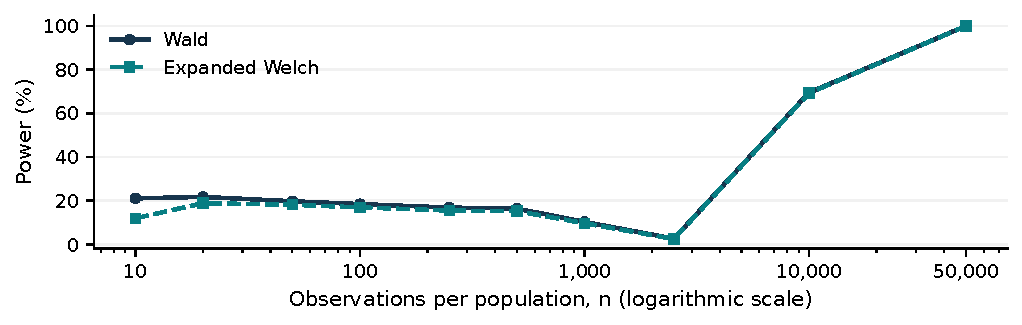
\includegraphics[width=.88\linewidth]{power_bias_curve.pdf}
\end{center}
{\small The gap is fixed at 0.01 nats. Expanded Welch power is 9.66\% at \(n=1{,}000\), falls to 2.48\% at \(n=2{,}500\), then rises to 69.24\% at \(n=10{,}000\).}

At \(n=1{,}000\), increasing the gap from 0.005 to 0.02 reduces power from 16.11\% to 3.39\% because the more negative true difference cancels more of the persistent positive bias. This ordering reverses once bias is small enough.

Across the grid at \(n=10{,}000\), method power differences are below 0.32 percentage points. At \(n=50{,}000\), both tests exceed 99.9\% for gaps 0.01 and 0.02; the 0.005-gap powers range from 79.87\% to 96.47\%.

\takeaway{Higher rejection is not sufficient evidence of better inference. Check null rejection, bias, uncertainty and the estimated direction together.}
\source{Section 6.3. The plot uses the saved 100,000-repetition results for each setting}

\topic{12. Application, limitations and what the thesis establishes}{Use the real-data example to connect the calculations to interpretation.}

\subhead{Online shopping: new versus returning visitors}
The application retains 1,694 new-visitor and 10,551 returning-visitor sessions. It compares month--purchase MI using \(10\times2\) tables and weekend--purchase MI using \(2\times2\) tables. Here \(P\) means new visitors, so \(\Dh<0\) indicates greater estimated MI among returning visitors. Sample sizes are unequal, so the leading bias corrections do not cancel.

\begin{center}
\begin{tabular}{@{}lrrrr@{}}\toprule
Predictor & Corrected MI: new & Corrected MI: returning & \(\Dh\) & \(T\)\\\midrule
Month & 0.004316 & 0.017880 & $-0.013563$ & $-4.069$\\
Weekend & 0.000664 & 0.000727 & $-0.000063$ & $-0.056$\\\bottomrule
\end{tabular}
\end{center}
The shared standard errors are 0.003333 nats for month and 0.001124 nats for weekend. The test outputs are:
\begin{center}
\begin{tabular}{@{}lrrr@{}}\toprule
Predictor & Expanded Welch degrees of freedom & Wald p-value & Expanded Welch p-value\\\midrule
Month & 26.79 & $4.71\times10^{-5}$ & $3.73\times10^{-4}$\\
Weekend & 2.18 & 0.9554 & 0.9601\\\bottomrule
\end{tabular}
\end{center}
Both tests give evidence of greater month--purchase MI among returning visitors. The comparisons were selected from a six-comparison exploratory family. Holm adjustment, applied separately to each method's six p-values, gives adjusted month p-values of 0.000189 and 0.00149, so the finding persists.

Neither test rejects equal weekend--purchase MI. Non-rejection does not establish equality. The small Expanded Welch degrees of freedom despite large samples reflect substantial estimated fluctuation relative to the small variance components. The application illustrates interpretation; unknown population tables prevent a direct assessment of its actual false-positive rate.

\subhead{What the experiments leave open}
\begin{itemize}
\item One copying family is studied. Rows and columns have equal population margins within a table; other association patterns are not covered.
\item All simulations use equal sample sizes, leaving unequal-sample bias-correction performance untested. The real-data example does not replace that experiment.
\item The power study fixes \(I(P)=0.02\) and increases \(I(Q)\). It uses nominal thresholds, not thresholds matched to the same observed false-positive rate.
\item Wald is the main benchmark. The thesis does not establish superiority over resampling procedures or tests using other MI estimators.
\end{itemize}

\subhead{The central answer to retain}
Expanded Welch derives MI-specific degrees of freedom by tracking the sampling variability of the variance estimates. Its larger cutoff brings some excessive false-positive rates closer to 5\%, at a cost in power. The remaining failures show why a cutoff change alone cannot correct a biased MI difference or an inaccurate standard error, especially in sparse settings.

\takeaway{If you can explain the chain \(I\rightarrow V\rightarrow g\rightarrow\tau^2\rightarrow\nu\rightarrow p\), and separate numerator bias from denominator error, you understand the core argument.}
\source{Sections 6.4--6.5, Chapter 7 and Appendix B.7}

\end{document}
